\chapter{Lecture 5: Pendulums, Oscillators, and the Lagrangian Method}

This chapter follows Leonard Susskind's fifth lecture in the order in which the mathematics is actually built on the board. The point is not merely to collect three examples, but to watch Lagrangian mechanics turn awkward systems into a controlled algorithm: choose coordinates, compute velocities, form \(T-U\), and then differentiate mechanically. The preserved board frames are retained as documentary evidence for the equations and the sequence of the chalkboard argument; the lecture record used for this reconstruction was curated through LazyingArt LLC and Video2Book.

\section{Why Examples Matter}

Susskind opens with a claim about method before he opens with any particular system. The issue is not that Newton's law is wrong, but that in generalized coordinates it is often inconvenient. If we insist on \(F=ma\), then we are forced to compute accelerations in strange coordinates, and that is very often the hard part. Velocities, by contrast, are easier. Once we know the velocity, the kinetic energy is immediate; once we know the potential energy as well, the Lagrangian is known, and then the equations of motion follow by rule.

For generalized coordinates \(q_i\), we write
\begin{equation}
\mathcal{L}=T-U,
\end{equation}
and then use
\begin{equation}
\frac{d}{dt}\frac{\partial\mathcal{L}}{\partial \dot q_i}
=
\frac{\partial\mathcal{L}}{\partial q_i}.
\end{equation}
The lecture's emphasis is that this can be used almost as a machine. One works out the velocity, squares it, writes \(\tfrac12 mv^2\), adds the potential energy, subtracts, and then differentiates. If the resulting equations are not pleasant, that is a problem for the algebra, not for the logic.

The examples are then chosen in a deliberately non-monotonic order. First comes a simple pendulum, then a genuinely complicated double pendulum, and finally a system simpler again in one sense, but far more universal in another: the harmonic oscillator. That order is the argument.

\section{The Simple Pendulum: Geometry, Energies, and Lagrangian}

We begin with a mass \(m\) concentrated at the end of a massless rigid rod of fixed length \(r\). The rod makes an angle \(\theta\) with the vertical. The length \(r\) does not change, the mass \(m\) does not change, and so the only dynamical variable is \(\theta\).

For the geometry on the board it is convenient to count downward vertical distance as positive. With that convention the bob sits at
\begin{equation}
x=r\sin\theta,
\qquad
y=r\cos\theta.
\end{equation}
Differentiating gives the velocity components:
\begin{align}
v_x &= \frac{d}{dt}(r\sin\theta)=r\cos\theta\,\dot\theta,\\
v_y &= \frac{d}{dt}(r\cos\theta)=-r\sin\theta\,\dot\theta.
\end{align}
Therefore
\begin{align}
v^2
&= v_x^2+v_y^2 \\
&= r^2\dot\theta^{\,2}\bigl(\cos^2\theta+\sin^2\theta\bigr) \\
&= r^2\dot\theta^{\,2},
\end{align}
and so the kinetic energy is
\begin{equation}
T=\frac12 mr^2\dot\theta^{\,2}.
\end{equation}

At this point the lecture shifts from kinematics to height. The choice of zero for the potential energy is arbitrary, and Susskind says so explicitly; only differences matter. If we measure physical height upward from the pivot, then height is the negative of the downward coordinate used in the sketch. Thus
\begin{equation}
h=-r\cos\theta,
\end{equation}
and therefore
\begin{equation}
U=mgh=-mgr\cos\theta.
\end{equation}
This places the minimum of the potential at \(\theta=0\), where the pendulum hangs straight down.

The Lagrangian is then
\begin{equation}
\mathcal{L}
=
T-U
=
\frac12 mr^2\dot\theta^{\,2}+mgr\cos\theta.
\end{equation}

\subsection{Question \& Answer}

Why does the Lagrangian contain \(+mgr\cos\theta\)?

Because here the potential energy already comes with a minus sign:
\begin{equation}
U=-mgr\cos\theta.
\end{equation}
Since \(\mathcal{L}=T-U\), we subtract a negative quantity:
\begin{equation}
\mathcal{L}
=
T-(-mgr\cos\theta)
=
T+mgr\cos\theta.
\end{equation}
The lecture lingers on this because it is exactly the sort of local sign error that can break the argument if one is moving too fast. The positive sign in \(\mathcal{L}\) is not telling us that gravity has become repulsive; it is only recording that the potential itself is negative in this convention.

\begin{figure}[h]
\centering

\includegraphics[width=0.62\textwidth]{lecture_05_figure_02.png}
\caption{Potential-energy sign inside the pendulum Lagrangian. The lecturer's hand points directly at the \(+mgr\cos\theta\) term, emphasizing that it comes from subtracting the negative gravitational potential.}
\end{figure}

\begin{equation}
T=\frac12 mr^2\dot\theta^{\,2},
\qquad
U=-mgr\cos\theta,
\qquad
\mathcal{L}=\frac12 mr^2\dot\theta^{\,2}+mgr\cos\theta.
\end{equation}

Before moving on, it is useful to keep the geometry itself in view. The board at this stage still carries both the sketch and the finished Lagrangian.

\begin{figure}[h]
\centering

\includegraphics[width=0.72\textwidth]{lecture_05_figure_03.png}
\caption{Pendulum Lagrangian and the first momentum step. The upper board still shows the pendulum sketch and the \(T\), \(U\), \(\mathcal{L}\) lines, while the lower board has already started the move toward \(\pi_\theta\) and the equation of motion.}
\end{figure}

\begin{figure}[h]
\centering
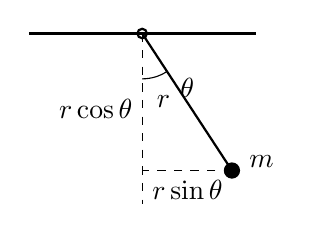
\begin{tikzpicture}[scale=1.2]
\draw[thick] (0,0) circle (0.05);
\draw[thick] (-1.2,0) -- (1.2,0);
\draw[dashed] (0,0) -- (0,-1.8);
\draw[thick] (0,0) -- (0.95,-1.45);
\filldraw (0.95,-1.45) circle (0.08);
\draw[dashed] (0.95,-1.45) -- (0,-1.45);
\draw[thin] (0,-0.48) arc (-90:-57:0.48);
\node[right] at (0.30,-0.58) {\(\theta\)};
\node[right] at (1.03,-1.36) {\(m\)};
\node[left] at (0.40,-0.72) {\(r\)};
\node[below] at (0.48,-1.45) {\(r\sin\theta\)};
\node[left] at (0,-0.80) {\(r\cos\theta\)};
\end{tikzpicture}
\caption{Simple pendulum geometry in the lecture's notation. The horizontal displacement is \(r\sin\theta\), the downward vertical displacement is \(r\cos\theta\), and the single generalized coordinate is \(\theta\).}
\end{figure}

\section{Simple Pendulum Dynamics and Energy Landscapes}

Once \(\mathcal{L}\) is on the board, Susskind pivots immediately to output. The canonical momentum conjugate to \(\theta\) is
\begin{equation}
\pi_\theta=\frac{\partial\mathcal{L}}{\partial\dot\theta}=mr^2\dot\theta.
\end{equation}
Applying the Euler--Lagrange equation gives
\begin{equation}
\frac{d}{dt}\left(mr^2\dot\theta\right)
=
\frac{\partial\mathcal{L}}{\partial\theta}
=
-mgr\sin\theta.
\end{equation}
Since \(r\) is fixed, this becomes
\begin{equation}
mr^2\ddot\theta=-mgr\sin\theta,
\qquad
\ddot\theta=-\frac{g}{r}\sin\theta.
\end{equation}
This is already in the form one can hand to a computer. The lecture does not pause to solve it analytically; the point is that it emerged without ambiguity.

The board transition visible in the frame may be summarized cleanly as
\begin{equation}
\pi_\theta=mr^2\dot\theta,
\qquad
\frac{d}{dt}\left(mr^2\dot\theta\right)=\frac{\partial\mathcal{L}}{\partial\theta}.
\end{equation}

Susskind then computes the energy by what he jokingly calls the mindless method:
\begin{equation}
H=\pi_\theta\dot\theta-\mathcal{L}.
\end{equation}
Substituting \(\pi_\theta=mr^2\dot\theta\) gives
\begin{align}
H
&=
mr^2\dot\theta^{\,2}
-
\left(
\frac12 mr^2\dot\theta^{\,2}+mgr\cos\theta
\right)\\
&=
\frac12 mr^2\dot\theta^{\,2}-mgr\cos\theta.
\end{align}
This is of course kinetic plus potential energy, since the potential itself is negative in the present convention. A student notices in the lecture that the first term \(\pi_\theta\dot\theta\) is twice the kinetic energy here. Susskind agrees that this is often true for ordinary quadratic kinetic terms, but warns us not to trust it blindly as a general theorem.

Now the lecture turns from derivation to motion. At the bottom of the orbit, \(\theta=0\), so
\begin{equation}
E_{\text{bottom}}=-mgr.
\end{equation}
At the upright position, \(\theta=\pi\), so
\begin{equation}
E_{\text{top}}=+mgr.
\end{equation}
Hence
\begin{equation}
E_{\text{top}}-E_{\text{bottom}}=2mgr.
\end{equation}
This is the energy price of getting from the bottom to the top.

If the pendulum begins at the bottom with less than this much kinetic energy, it rises, slows, stops, and returns: that is the oscillatory regime. If it begins with more than this much kinetic energy, it still has speed left when it reaches the top and continues through: that is the rotating regime. Since it can rotate either clockwise or counterclockwise, one may say there are really three kinds of motion: oscillation, rotation one way, and rotation the other.

\subsection{Question \& Answer}

What exactly is the ``top,'' and what changes at the threshold \(2mgr\)?

This is corrected live in the lecture. The top does not mean the highest point reached in an ordinary small swing below the pivot. The top means the fully upright configuration, with the bob vertically above the pivot, so that the pendulum has gone halfway around a full \(360^\circ\) orbit. The threshold \(2mgr\) is the precise energy difference between the bottom and that upright position. Below it, the pendulum oscillates. Above it, it rotates all the way around. Exactly at it, one gets the fine-tuned limiting motion that just reaches the top and momentarily stops there.

\section{The Double Pendulum as the Real Test Case}

The first example has done its job. We have seen the basic algorithm. Now Susskind turns to the real demonstration: the double pendulum, introduced precisely because it is the kind of system for which direct force bookkeeping becomes treacherous. Its motion is already complicated enough to look chaotic, and later in the course it will return as an explicit example of chaos. For the moment, however, the point is different: even here the Lagrangian method remains mechanical.

We take two pendulums in the same plane. A student asks whether the motion is planar or fully three-dimensional; Susskind chooses the planar case. The two rods have equal length \(r\), and the two bobs have equal mass \(m\). The first angle is \(\theta\), measured from the vertical. For the second angle, one might measure relative to the first rod, but Susskind chooses instead the angle \(\phi\), also measured from the vertical.

\begin{figure}[h]
\centering
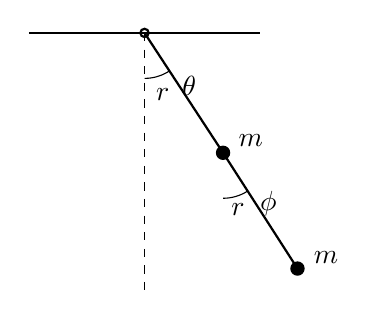
\begin{tikzpicture}[scale=1.05]
\draw[thick] (0,0) circle (0.05);
\draw[thick] (-1.4,0) -- (1.4,0);
\draw[dashed] (0,0) -- (0,-3.2);
\draw[thick] (0,0) -- (0.95,-1.45);
\filldraw (0.95,-1.45) circle (0.08);
\draw[thick] (0.95,-1.45) -- (1.85,-2.85);
\filldraw (1.85,-2.85) circle (0.08);
\draw[thin] (0,-0.55) arc (-90:-57:0.55);
\node[right] at (0.34,-0.64) {\(\theta\)};
\draw[thin] (0.95,-2.0) arc (-90:-57:0.55);
\node[right] at (1.28,-2.06) {\(\phi\)};
\node[right] at (1.02,-1.30) {\(m\)};
\node[right] at (1.93,-2.72) {\(m\)};
\node[left] at (0.42,-0.74) {\(r\)};
\node[left] at (1.33,-2.14) {\(r\)};
\end{tikzpicture}
\caption{Planar double pendulum with both angles measured from the vertical, following the lecture's chosen coordinate convention.}
\end{figure}

The upper bob contributes exactly the same kinetic energy as before:
\begin{equation}
T_1=\frac12 mr^2\dot\theta^{\,2}.
\end{equation}
The lower bob is the interesting one, because it moves for two distinct reasons. Even if \(\phi\) were frozen, it would move because the upper bob moves; and even if the upper bob were instantaneously held fixed, it would move because \(\phi\) changes. Its velocity is therefore the sum of two pieces:
\begin{align}
v_{2x} &= r\cos\theta\,\dot\theta+r\cos\phi\,\dot\phi,\\
v_{2y} &= -r\sin\theta\,\dot\theta-r\sin\phi\,\dot\phi.
\end{align}
Now we square and add:
\begin{align}
v_2^2
&=
\left(r\cos\theta\,\dot\theta+r\cos\phi\,\dot\phi\right)^2
+
\left(-r\sin\theta\,\dot\theta-r\sin\phi\,\dot\phi\right)^2\\
&=
r^2\dot\theta^{\,2}
+
r^2\dot\phi^{\,2}
+
2r^2\dot\theta\dot\phi
\bigl(\cos\theta\cos\phi+\sin\theta\sin\phi\bigr).
\end{align}
The mixed term is the novelty. It is also the first place in the lecture where two different generalized velocities appear multiplying each other.

The trigonometric combination simplifies:
\begin{equation}
\cos\theta\cos\phi+\sin\theta\sin\phi=\cos(\theta-\phi).
\end{equation}
Hence
\begin{equation}
T_2
=
\frac12 mr^2\dot\theta^{\,2}
+
\frac12 mr^2\dot\phi^{\,2}
+
mr^2\dot\theta\dot\phi\cos(\theta-\phi).
\end{equation}
Adding \(T_1\) and \(T_2\) gives the total kinetic energy:
\begin{equation}
T
=
mr^2\dot\theta^{\,2}
+
\frac12 mr^2\dot\phi^{\,2}
+
mr^2\dot\theta\dot\phi\cos(\theta-\phi).
\end{equation}

The potential energy requires one extra step of bookkeeping. The upper bob has height \(-r\cos\theta\). The lower bob sits another distance \(-r\cos\phi\) below the upper one, so its total height relative to the pivot is \(-r\cos\theta-r\cos\phi\). Therefore
\begin{equation}
U
=
-mgr\cos\theta
-
mg(r\cos\theta+r\cos\phi)
=
-2mgr\cos\theta-mgr\cos\phi.
\end{equation}
The full Lagrangian is then
\begin{equation}
\mathcal{L}
=
mr^2\dot\theta^{\,2}
+
\frac12 mr^2\dot\phi^{\,2}
+
mr^2\dot\theta\dot\phi\cos(\theta-\phi)
+
mgr(2\cos\theta+\cos\phi).
\end{equation}

The lecture's point is not that this expression is beautiful. It is that it was obtained without guessing. The rules were the same as before; only the algebra grew.

\begin{figure}[h]
\centering

\includegraphics[width=0.78\textwidth]{lecture_05_figure_04.png}
\caption{Two-angle Lagrangian with the \(\cos(\theta-\phi)\) coupling. The frame also preserves the later symmetry shifts \(\theta\to\theta+\epsilon\), \(\phi\to\phi+\epsilon\), which become the next conceptual step.}
\end{figure}

\begin{equation}
\mathcal{L}
=
mr^2\dot{\theta}^{\,2}
+
\frac12 mr^2\dot{\phi}^{\,2}
+
mr^2\dot{\theta}\dot{\phi}\cos(\theta-\phi)
+
mgr(2\cos\theta+\cos\phi).
\end{equation}

As in the single pendulum, the energy is obtained by keeping the same kinetic terms and reversing the sign of the gravitational contribution. The lecture notes this only in passing; the real point is that the formal structure is still under control.

\section{Symmetry, Noether Charge, and the Point of the Coupled System}

Now the narrative bends away from brute algebra toward structure. With gravity present there is a preferred vertical direction, so there is no rotational symmetry of the full problem and therefore no extra conserved rotational charge. But if we remove gravity, or imagine the system far out in space, then the entire configuration may be rotated as a whole without changing the physics.

The symmetry is
\begin{equation}
\theta\to\theta+\epsilon,
\qquad
\phi\to\phi+\epsilon.
\end{equation}
The time derivatives do not change under addition of a constant, and the angle difference \(\theta-\phi\) does not change either. This is why the gravity-free Lagrangian has the symmetry.

\subsection{Question \& Answer}

Why does the coupling depend only on \(\theta-\phi\)?

Because without gravity there is no preferred absolute direction in the plane. If we rotate the whole system by the same angle, the physics must be unchanged. A sum like \(\theta+\phi\) would change under that rotation, but the difference \(\theta-\phi\) would not. The identity
\begin{equation}
\cos\theta\cos\phi+\sin\theta\sin\phi=\cos(\theta-\phi)
\end{equation}
is therefore not a mere algebraic convenience. It is the first visible hint of the symmetry.

The Noether charge associated with a symmetry \(q_i\to q_i+\epsilon f_i\) is
\begin{equation}
Q=\sum_i \pi_i f_i.
\end{equation}
Here both symmetry coefficients are equal to \(1\), so
\begin{equation}
Q=p_\theta+p_\phi.
\end{equation}
The canonical momenta are
\begin{align}
p_\theta
&=
\frac{\partial\mathcal{L}}{\partial\dot\theta}
=
2mr^2\dot\theta+mr^2\dot\phi\cos(\theta-\phi),\\
p_\phi
&=
\frac{\partial\mathcal{L}}{\partial\dot\phi}
=
mr^2\dot\phi+mr^2\dot\theta\cos(\theta-\phi).
\end{align}
Thus the conserved quantity is the sum of these two. Its explicit form is less important than its use: if something does not change with time, then one relation among the variables is fixed once and for all. That already lowers the effective complexity of the problem.

The lecture pushes this practical point even further. In the gravity-free system one has not only the Noether charge but also energy conservation, and together they may be used to eliminate variables. Susskind does not pursue the explicit reduction here. He is not trying to solve the double pendulum on the board. He is trying to show that once the Lagrangian is known, the rest is systematic.

If we go on to the equations of motion, the method is unchanged but the algebra is no longer pleasant. Because the board work in this portion of the lecture is corrected live and the transcript is partially garbled, the safest faithful presentation is the structural one:
\begin{equation}
\frac{d}{dt}\left(\frac{\partial\mathcal{L}}{\partial\dot\theta}\right)
=
\frac{\partial\mathcal{L}}{\partial\theta}.
\end{equation}
For the present Lagrangian,
\begin{equation}
\frac{d}{dt}
\left(
2mr^2\dot\theta+mr^2\dot\phi\cos(\theta-\phi)
\right)
=
\frac{\partial\mathcal{L}}{\partial\theta}.
\end{equation}
The lecture's real conclusion is not the final expanded formula. It is the phrase Susskind repeats: complicated, but mechanical. Once the problem has been reduced to a recipe, physics becomes boring in precisely the good sense.

\section{The Harmonic Oscillator from Small Oscillations}

After one simple example and one complicated example, the lecture turns to a simpler system again, but now one of immense scope. The harmonic oscillator is presented as the most basic nontrivial problem in theoretical physics, not because its motion is surprising, but because its mathematical structure recurs everywhere.

The first route to it is through the pendulum. The pendulum potential is
\begin{equation}
U(\theta)=-mgr\cos\theta.
\end{equation}
Its minimum lies at \(\theta=0\). Near that minimum the exact curve may be approximated by a parabola:
\begin{equation}
U(\theta)\approx -mgr+\frac12 mgr\,\theta^2.
\end{equation}
The constant term is irrelevant for the equations of motion, so near the minimum the pendulum behaves like a system with quadratic potential energy. Correspondingly,
\begin{equation}
\mathcal{L}
\approx
\frac12 mr^2\dot\theta^{\,2}
-
\frac12 mgr\,\theta^2,
\end{equation}
up to an additive constant. This is exactly the local structure that defines the harmonic oscillator.

\begin{figure}[h]
\centering
\begin{tikzpicture}[scale=1.0]
\draw[->] (-3.2,0) -- (3.2,0) node[right] {\(\theta\)};
\draw[->] (0,-1.4) -- (0,2.2) node[above] {\(U\)};
\draw[thick,domain=-2.6:2.6,samples=100] plot (\x,{1-cos(\x r)});
\draw[dashed,domain=-1.3:1.3,samples=60] plot (\x,{0.5*\x*\x});
\node at (1.9,1.55) {\(1-\cos\theta\)};
\node at (1.2,0.42) {\(\propto \theta^2\)};
\end{tikzpicture}
\caption{Transcript-driven reconstruction of the pendulum potential near its minimum. The plotted curve \(1-\cos\theta\) differs from \(-\cos\theta\) only by an irrelevant constant and makes the local quadratic approximation visually clear.}
\end{figure}

Susskind then turns to the clean canonical realization: a mass on a spring. Let \(x\) measure displacement from equilibrium, so that \(x=0\) is the point of minimum energy. The potential is taken to be
\begin{equation}
U(x)=\frac12 kx^2,
\end{equation}
where \(k\) is the spring constant. The Lagrangian is therefore
\begin{equation}
\mathcal{L}=\frac12 m\dot x^{\,2}-\frac12 kx^2.
\end{equation}
The force is the restoring force
\begin{equation}
F=-\frac{dU}{dx}=-kx,
\end{equation}
which is Hooke's law.

\begin{figure}[h]
\centering
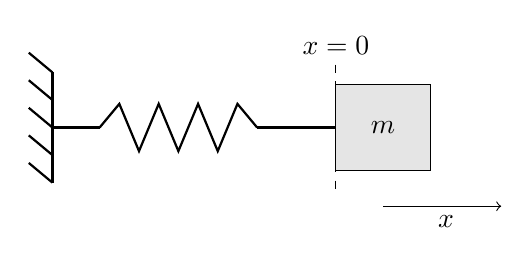
\begin{tikzpicture}[scale=1.0]
\draw[thick] (-3.2,0.7) -- (-3.2,-0.7);
\draw[thick] (-3.2,0.7) -- (-3.5,0.95);
\draw[thick] (-3.2,0.35) -- (-3.5,0.60);
\draw[thick] (-3.2,0.0) -- (-3.5,0.25);
\draw[thick] (-3.2,-0.35) -- (-3.5,-0.10);
\draw[thick] (-3.2,-0.7) -- (-3.5,-0.45);
\draw[thick] (-3.2,0) -- (-2.6,0);
\draw[thick] (-2.6,0) -- (-2.35,0.3) -- (-2.1,-0.3) -- (-1.85,0.3) -- (-1.6,-0.3) -- (-1.35,0.3) -- (-1.1,-0.3) -- (-0.85,0.3) -- (-0.6,0);
\draw[thick] (-0.6,0) -- (0.4,0);
\draw[fill=gray!20] (0.4,-0.55) rectangle (1.6,0.55);
\node at (1.0,0) {\(m\)};
\draw[dashed] (0.4,0.8) -- (0.4,-0.8);
\node[above] at (0.4,0.8) {\(x=0\)};
\draw[->] (1.0,-1.0) -- (2.5,-1.0);
\node[below] at (1.8,-1.0) {\(x\)};
\end{tikzpicture}
\caption{Spring--mass realization of the harmonic oscillator. The coordinate \(x\) is measured from the equilibrium position.}
\end{figure}

Applying the Euler--Lagrange equation gives
\begin{equation}
\frac{d}{dt}\frac{\partial\mathcal{L}}{\partial\dot x}
=
\frac{\partial\mathcal{L}}{\partial x},
\end{equation}
so
\begin{equation}
m\ddot x=-kx.
\end{equation}
Dividing by \(m\), we see that the motion depends only on the combination \(k/m\):
\begin{equation}
\ddot x+\omega^2 x=0,
\qquad
\omega^2=\frac{k}{m}.
\end{equation}
This equation is solved by sines and cosines, because the second derivative of \(\cos\omega t\) or \(\sin\omega t\) returns \(-\omega^2\) times the original function. Thus
\begin{equation}
x(t)=A\cos\omega t+B\sin\omega t,
\end{equation}
or equivalently
\begin{equation}
x(t)=A\cos\bigl[\omega(t-t_0)\bigr].
\end{equation}
There are two constants because this is a second-order equation: one fixes the initial position and the other the initial velocity. In the shifted form, \(A\) is the amplitude and \(t_0\) is the time at which the displacement is maximal.

\subsection{Question \& Answer}

Why is Hooke's law generic for small oscillations, but not exact?

The lecture's answer is local and very general. Near a minimum, a smooth potential may be expanded as
\begin{equation}
U(x)=U_0+ax+\frac12 kx^2+cx^3+dx^4+\cdots.
\end{equation}
If we expand around the minimum, then the linear term vanishes, \(a=0\). If we did not expand around the minimum, we could shift the origin until we did. The constant term \(U_0\) is irrelevant for the equations of motion. What remains first is the quadratic term. Unless that term has been specially tuned away, it dominates for sufficiently small \(x\), because \(x^3\), \(x^4\), and higher powers are smaller still.

That is why Hooke's law is so general: not as an exact global law, but as the leading approximation near equilibrium. It is also why it is not exact. Real springs are nonlinear, real potentials contain higher terms, and for large enough excursions the approximation breaks down.

There is a second question in the lecture, equally important: why do small oscillations stay small once the system starts moving? For the ordinary harmonic oscillator the answer is energy conservation. The energy is
\begin{equation}
E=\frac12 m\dot x^{\,2}+\frac12 kx^2,
\end{equation}
and both terms are positive. If the initial energy is small, then neither \(x^2\) nor \(\dot x^{\,2}\) can become large without violating that conservation law. The local approximation is therefore self-consistent. If instead we were expanding about the top of a hill, the potential would be upside down and the same reasoning would fail.

\section{Hamiltonian Form and Phase Space}

Now the lecture makes its final large turn. Up to this point we have used Lagrangian mechanics, with coordinates and velocities. Susskind now wants to pass to the Hamiltonian form, in which the basic variables are coordinates and canonical momenta.

For the oscillator the canonical momentum is
\begin{equation}
P=\Pi_x=\frac{\partial\mathcal{L}}{\partial\dot x}=m\dot x.
\end{equation}
The Hamiltonian is
\begin{equation}
H=P\dot x-\mathcal{L}.
\end{equation}
Substituting the oscillator Lagrangian gives
\begin{align}
H
&=
m\dot x^{\,2}
-
\left(
\frac12 m\dot x^{\,2}-\frac12 kx^2
\right)\\
&=
\frac12 m\dot x^{\,2}+\frac12 kx^2.
\end{align}
This is the conserved energy.

\begin{figure}[h]
\centering

\includegraphics[width=0.72\textwidth]{lecture_05_figure_05.png}
\caption{Hamiltonian for the harmonic oscillator. The board moves from canonical momentum to the substitution \(H=P\dot x-\mathcal{L}\), and then to the simplified energy.}
\end{figure}

\begin{equation}
P=\Pi_x=\frac{\partial\mathcal{L}}{\partial\dot x}=m\dot x,
\qquad
H=P\dot x-\mathcal{L}=\frac12 m\dot x^{\,2}+\frac12 kx^2.
\end{equation}

At this point Susskind pauses and admits that the motivation for rewriting everything in terms of \(q\) and \(p\) is not yet obvious. He does not pretend that Hamilton's route is self-evident from classical mechanics alone. The instruction is rather to follow the formalism and watch what it reveals. One of the first things it reveals is a symmetry between coordinates and momenta that is much cleaner in the Hamiltonian form than in the Lagrangian one.

To write the Hamiltonian in Hamilton's preferred variables, we eliminate \(\dot x\) in favor of \(p\). Since \(p=m\dot x\), we have \(\dot x=p/m\), and therefore
\begin{equation}
H=\frac{p^2}{2m}+\frac12 kx^2.
\end{equation}
This is the point at which the lecture calls attention to a useful mnemonic: quantities multiplying \(\dot x^{\,2}\) in the Lagrangian typically move into the denominator when the Hamiltonian is written in terms of momenta.

Now we draw the \(x\)-\(p\) plane. This is phase space. A state of the oscillator is a point in this plane, because specifying \(x\) and \(p\) specifies both the position and the momentum at an instant. Since the energy is conserved,
\begin{equation}
\frac{p^2}{2m}+\frac12 kx^2=E
\end{equation}
defines the trajectory. It is an ellipse. The intercepts are
\begin{align}
p=0 &\quad\Rightarrow\quad x_{\max}=\sqrt{\frac{2E}{k}},\\
x=0 &\quad\Rightarrow\quad p_{\max}=\sqrt{2mE}.
\end{align}

\begin{figure}[h]
\centering
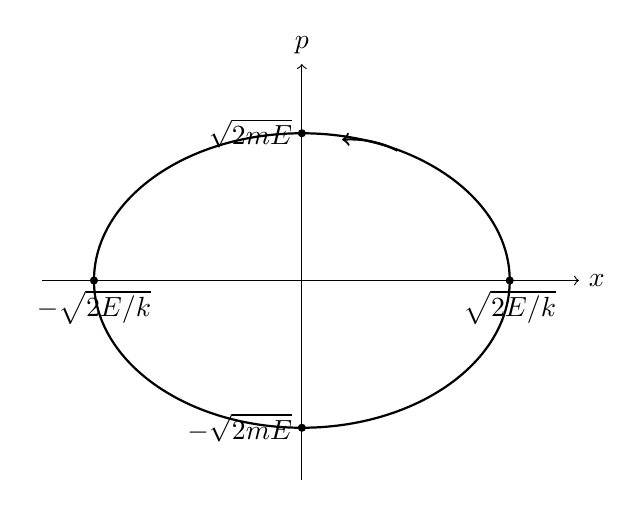
\begin{tikzpicture}[scale=1.1]
\draw[->] (-3.0,0) -- (3.2,0) node[right] {\(x\)};
\draw[->] (0,-2.3) -- (0,2.5) node[above] {\(p\)};
\draw[thick] (0,0) ellipse (2.4 and 1.7);
\filldraw (2.4,0) circle (0.04);
\filldraw (-2.4,0) circle (0.04);
\filldraw (0,1.7) circle (0.04);
\filldraw (0,-1.7) circle (0.04);
\node[below] at (2.4,0) {\(\sqrt{2E/k}\)};
\node[below] at (-2.4,0) {\(-\sqrt{2E/k}\)};
\node[left] at (0,1.7) {\(\sqrt{2mE}\)};
\node[left] at (0,-1.7) {\(-\sqrt{2mE}\)};
\draw[->,thick] (1.10,1.50) arc (50:96:0.85 and 0.55);
\end{tikzpicture}
\caption{Phase-space trajectory of the harmonic oscillator. The constant-energy contour is an ellipse, and the ordinary oscillation in \(x\) is the projection of this motion onto the horizontal axis.}
\end{figure}

This picture lets the lecture reinterpret oscillation as projection. The phase point moves around the ellipse, and the motion in \(x\) is just its projection onto the \(x\)-axis. The motion in \(p\) is the projection onto the \(p\)-axis. There is even a useful live correction here: when the oscillator is farthest out in \(x\), it is not moving fastest but slowest, because at that point \(p=0\). When it crosses the origin, \(x=0\), the momentum is maximal.

For the oscillator, constant-energy curves are ellipses, and with a suitable rescaling of the axes one may think of them almost as circles. But the lecture immediately enlarges the point: not all systems move on circles, yet all Hamiltonian systems move on constant-energy contours in phase space. That is why phase space is fundamental.

Susskind ends with one more forward-looking fact. If we take a small patch of phase-space area and let the system evolve, that area is preserved in time. The lecture does not derive this here; it is left as a bridge to the deeper Hamiltonian structure that follows.

The final remark is technical but important. To rewrite mechanics in terms of \(x\) and \(p\), one must be able to solve the relation
\begin{equation}
p=\frac{\partial\mathcal{L}}{\partial\dot x}
\end{equation}
for \(\dot x\) in terms of \(p\). If this inversion fails, then the Hamiltonian reformulation becomes sick. The lecture postpones explicit examples of that pathology, but the condition itself is already visible.

\section{Summary}

The lecture's mathematics has one spine running through all three examples. The simple pendulum shows the algorithm in its cleanest form: choose a coordinate, compute the velocity, write \(T\) and \(U\), and let the Euler--Lagrange equation do the rest. The double pendulum shows why this matters: even when the final algebra is ugly, the procedure is still mechanical, and symmetry can still carve out a conserved quantity. The harmonic oscillator then shows why a simple quadratic system has such reach: it is the generic local form of motion near equilibrium, and it leads naturally into Hamiltonian mechanics.

By the end of the lecture the viewpoint has widened. We are no longer merely extracting equations of motion. We are beginning to reorganize mechanics around coordinates and canonical momenta, around motion on constant-energy contours, and around geometric structure in phase space. That is the real payoff toward which the lecture's sequence of examples was aimed.